\chapter{Additional Figures}

\begin{figure}[ht!]
\centering
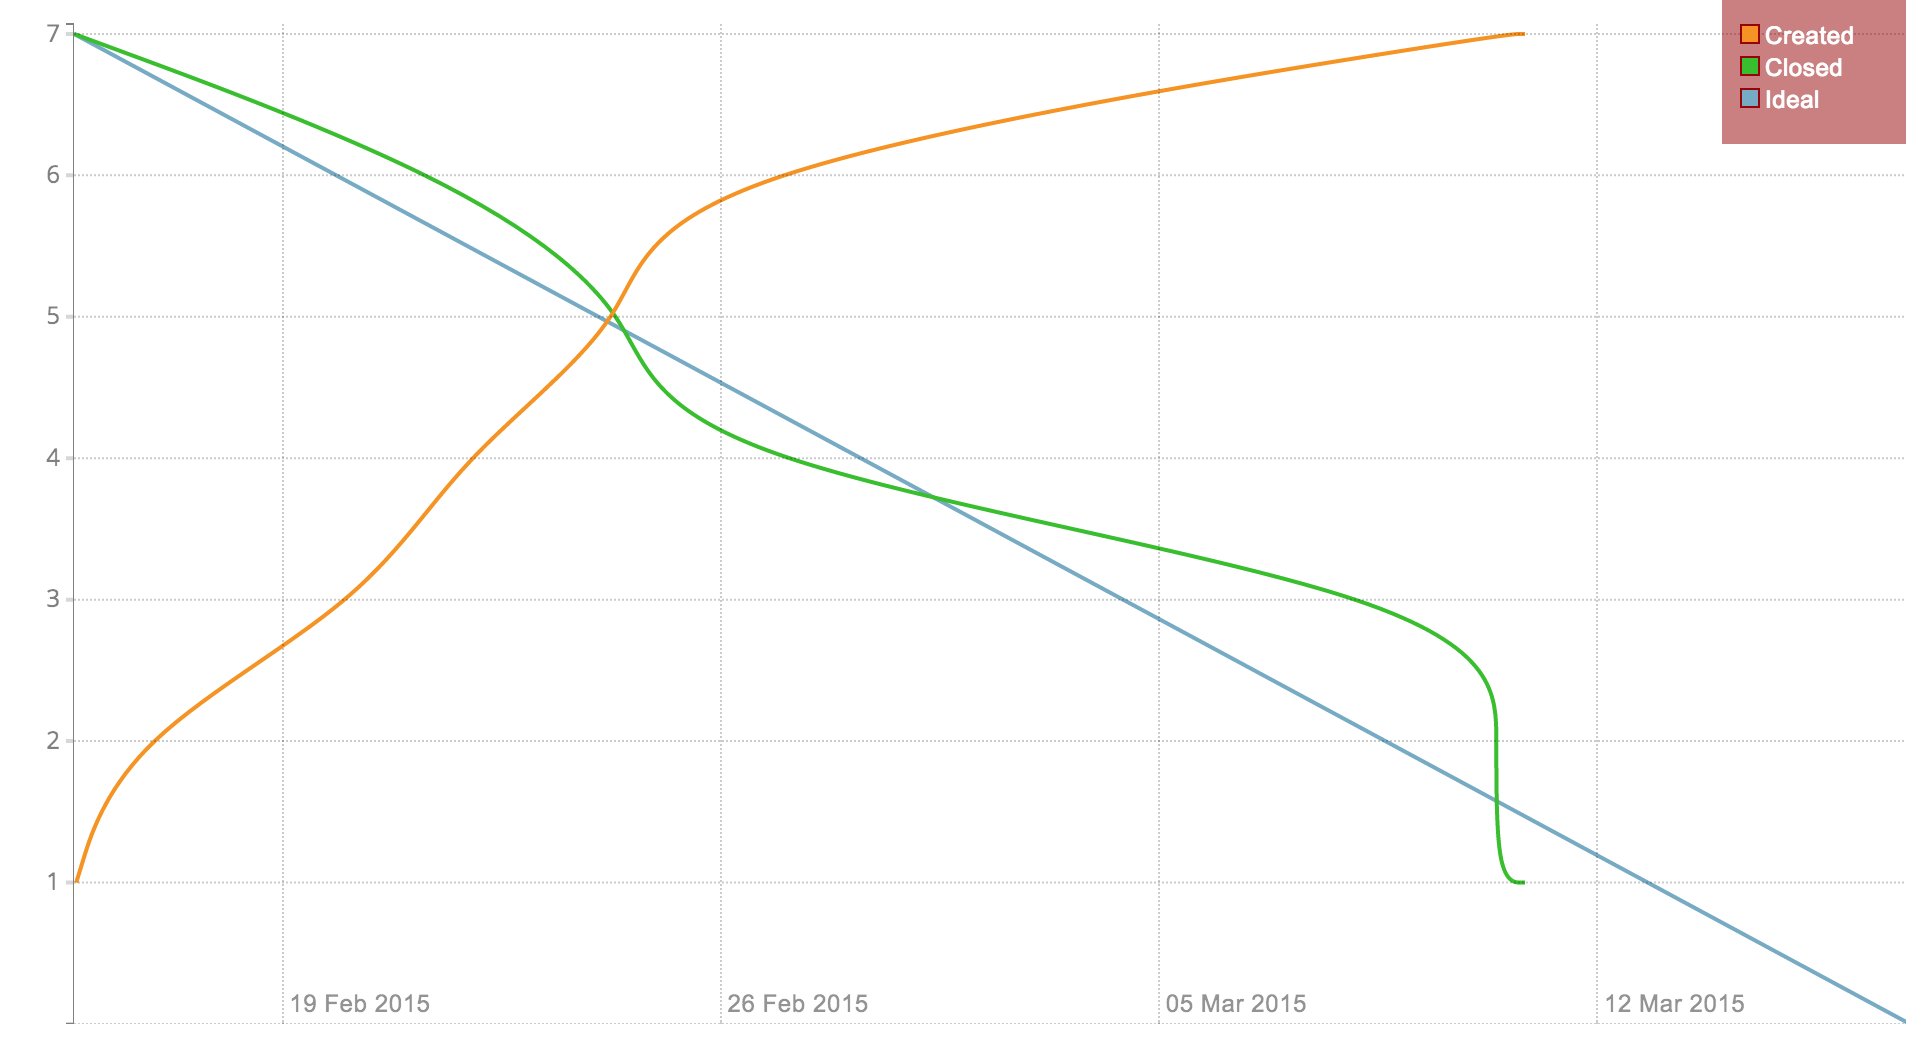
\includegraphics[scale=0.4]{images/burndown.png}
  \caption{Burndown chart indicating project progress over the previous 90-day period. Courtesy: \protect\url{http://burndown.io/#cgddrd/cs39440-major-project}.}
\label{fig:burndown}
\end{figure} 

\begin{figure}[ht!]
\centering
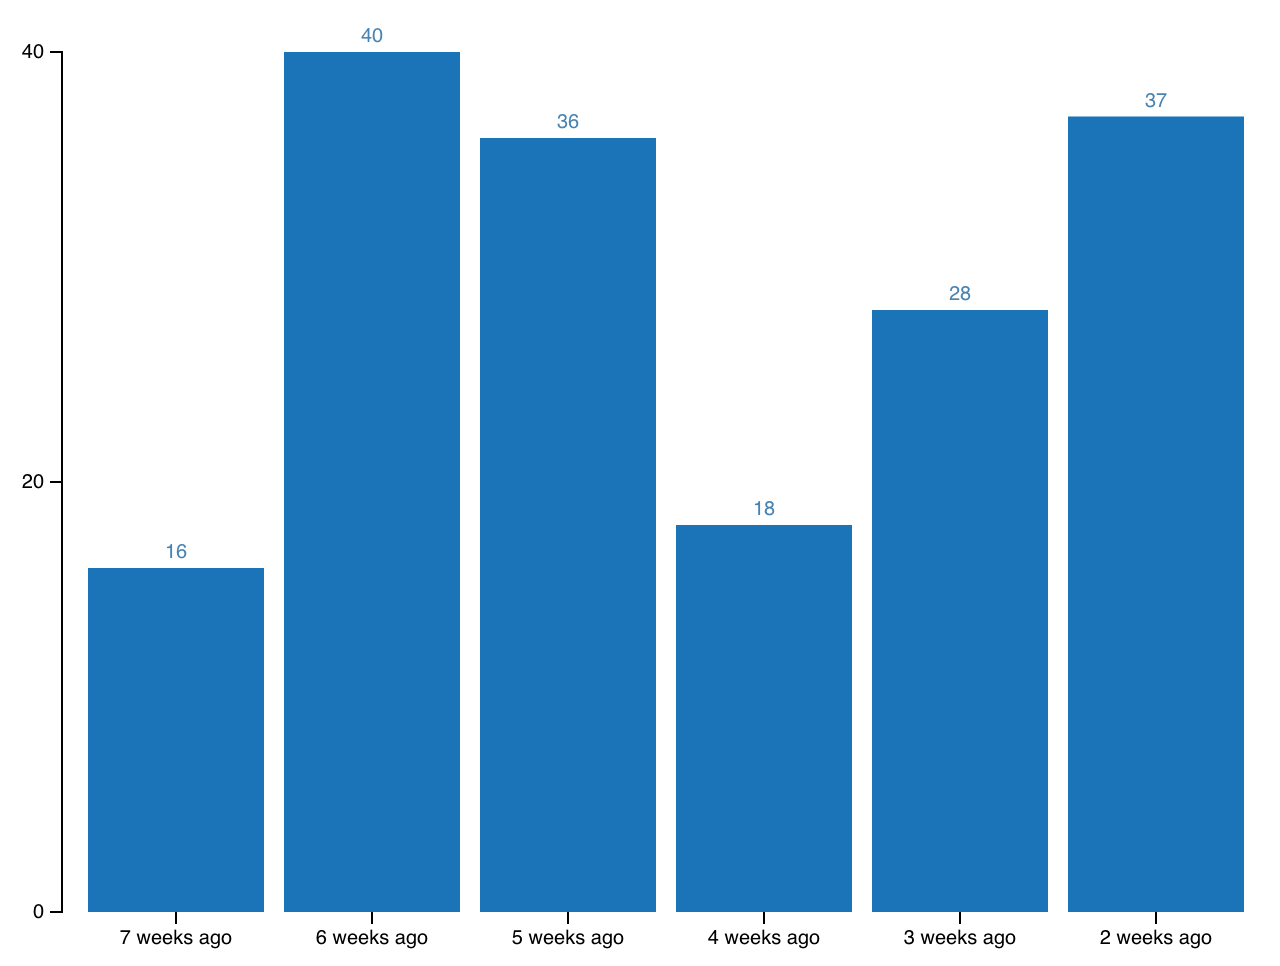
\includegraphics[scale=0.5]{images/throughput.png}
  \caption{Throughput chart describing rate of task completion in terms of task weighting over the previous eight weeks. Courtesy: \protect\url{https://waffle.io/cgddrd/cs39440-major-project/metrics/throughput}.}
\label{fig:throughput}
\end{figure} 

\begin{landscape}

	\begin{figure}[ht!]
\centering
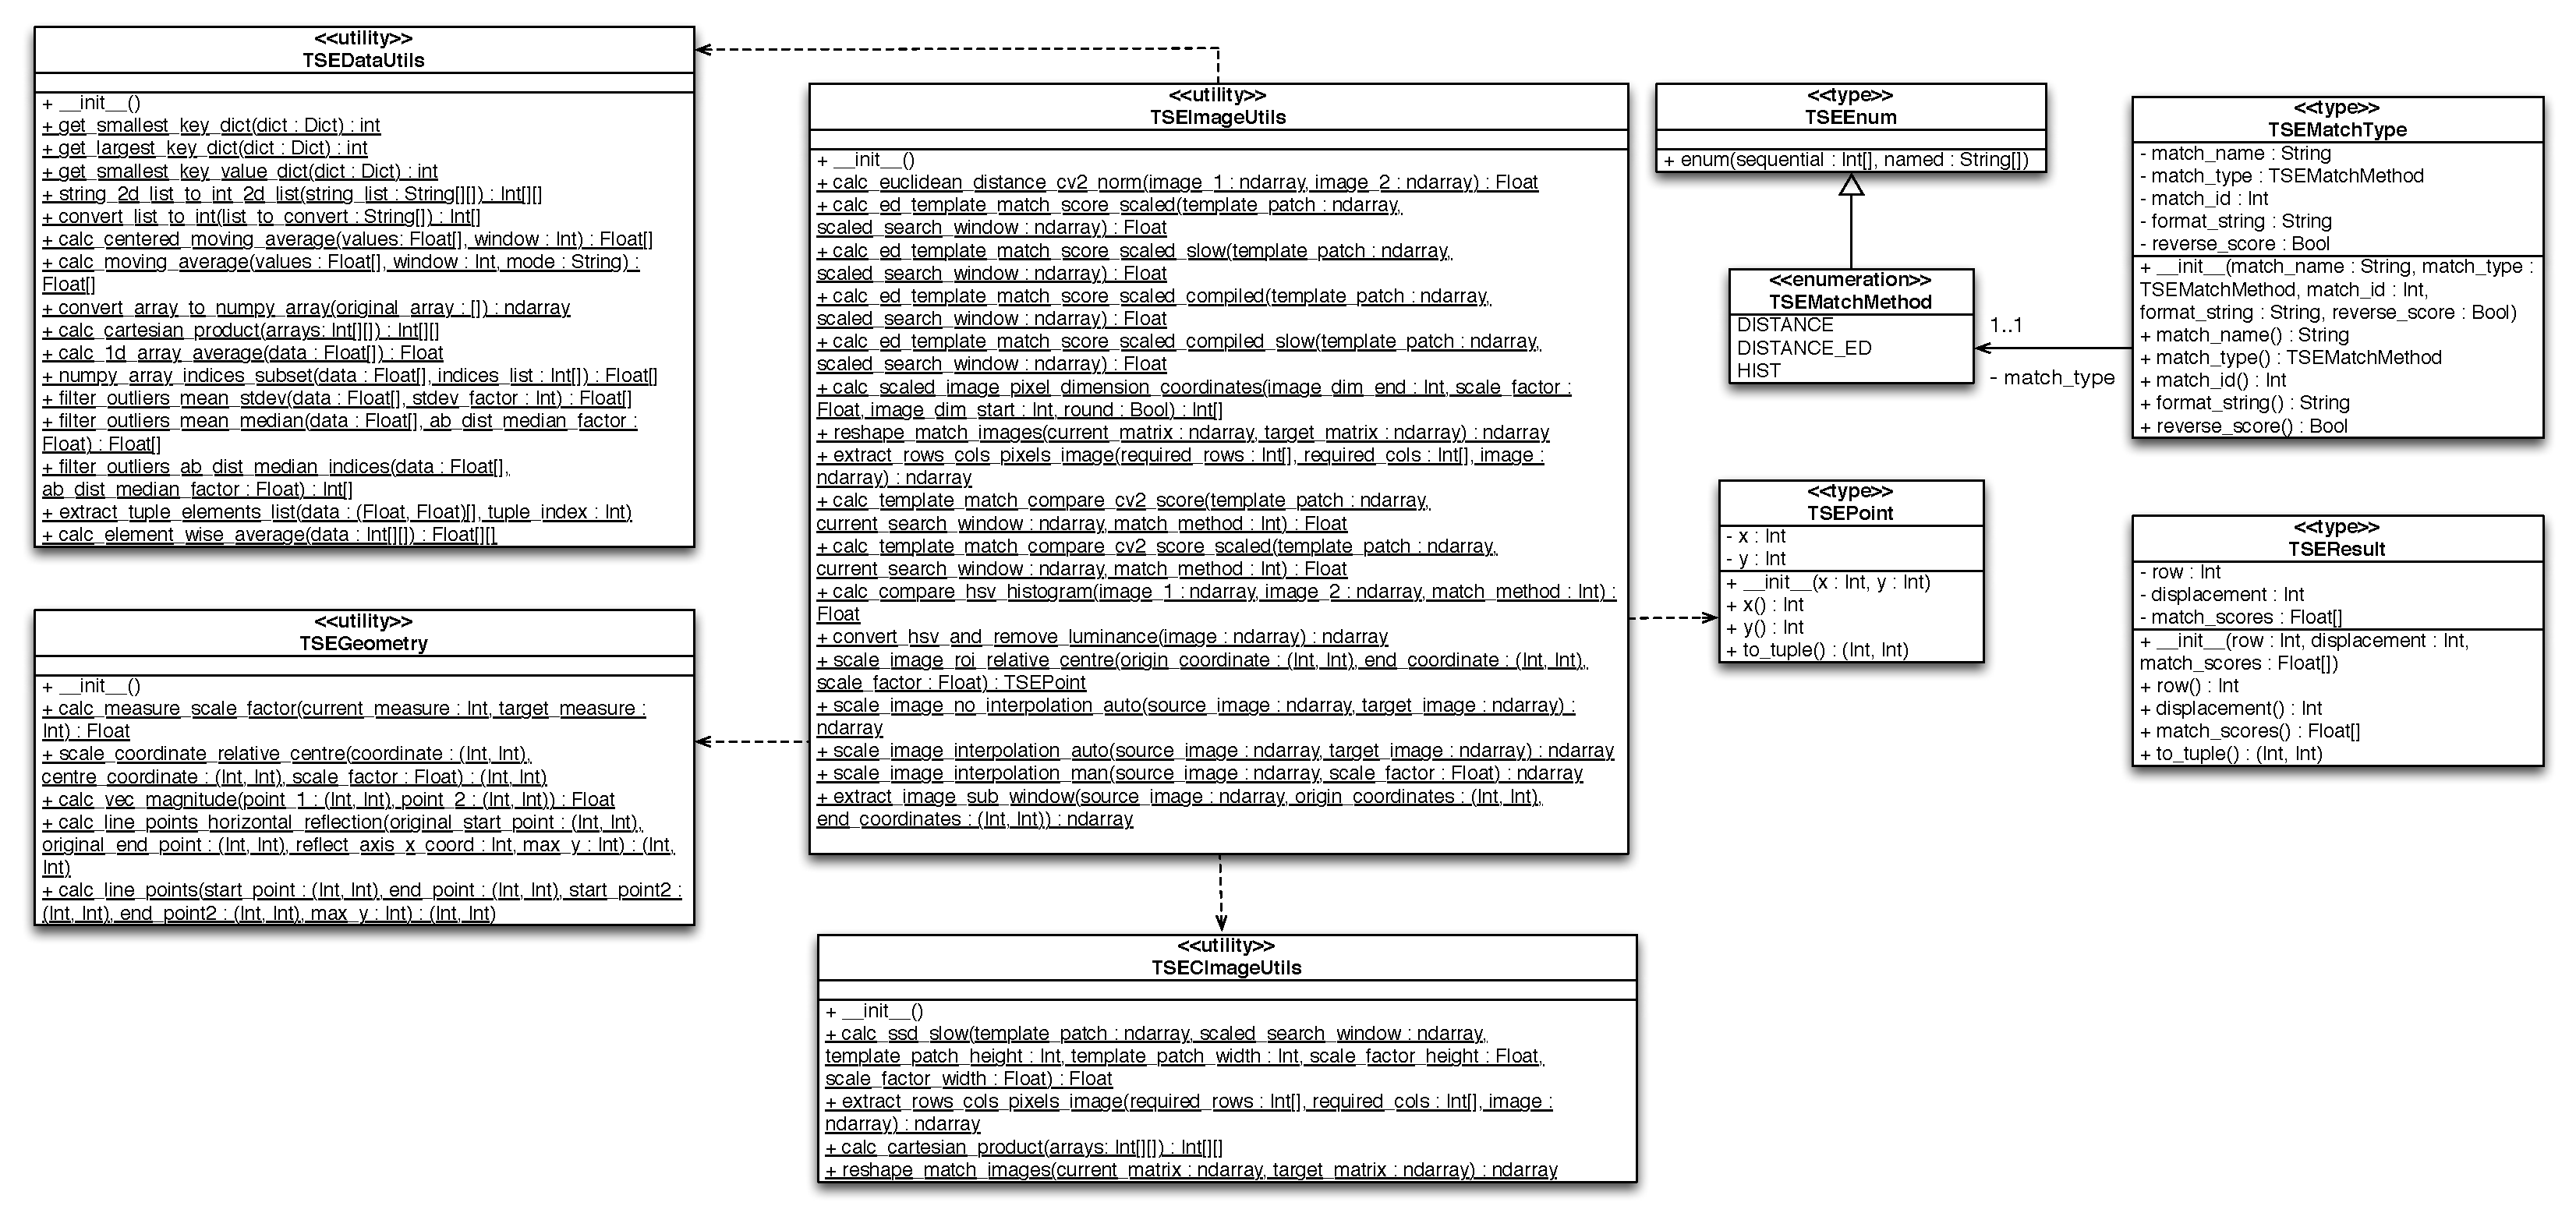
\includegraphics[scale=0.38]{images/tse_class_diagram}
  \caption{UML class diagram describing the structure of the `Terrain Shape Estimation'  Python-based library utilised extensively throughout the investigation for providing common functionality shared across experiments.}
\label{fig:class}
\end{figure} 

\end{landscape}


